\documentclass[a4paper]{article}
\usepackage[latin1, utf8]{inputenc}
\usepackage{graphicx}
\usepackage[francais]{babel}
%\usepackage[english,french]{babel}
\usepackage{amsmath}
\usepackage{amssymb}
\usepackage{mathrsfs}
\usepackage{multicol}
\usepackage{xcolor}
\usepackage[top=2.5cm, bottom=2.5cm, left=2cm, right=2cm]{geometry}
\usepackage{fancyhdr}
\lhead{\bsc{CE321}}
\rhead{\bsc{Challenge Entreprise}}
\renewcommand{\headrulewidth}{1px}
\lfoot{ \bsc{Enseirb-Matmeca}}
\rfoot{ \bsc{I3 - Robot}}
\renewcommand{\footrulewidth}{1px}
\pagestyle{fancy}
\usepackage[colorlinks=true,linkcolor=black,urlcolor=blue]{hyperref}
\usepackage{soul}
%\usepackage{wrapfig}
%\usepackage{framed}
%\usepackage[vlined,lined,boxed,french,longend]{algorithm2e}


%%%%%%%%%%%%%%%% Variables %%%%%%%%%%%%%%%%
\def\projet{Rapport d'activité}
\def\titre{ArchMobile}
%\def\groupe{2}
%\def\equipe{4}
%\def\responsible{classerre}
%\def\secretary{ahavlicek}
\def\others{lhofer, tlambert, classerre, lleclech}

\graphicspath{{graphics}{data/}}

\begin{document}
%%%%%%%%%%%%%%%% Header %%%%%%%%%%%%%%%%
\noindent\begin{minipage}{\textwidth}
\vskip 0mm
\noindent
    { \begin{tabular}{p{7.5cm}}
        {\bfseries \sffamily
          Projet \projet}
        \begin{center}{\itshape \titre}\end{center}
    \end{tabular}}
    \hfill 
    \fbox{\begin{tabular}{l}
        {~\hfill \bfseries \sffamily \others}
    \end{tabular}}
    \vskip 4mm ~

    ~~~\parbox{0.95\textwidth}{\small \textit{Résumé~:} \sffamily
      Le but de ce projet...
}
      
    \vskip 1mm ~
\end{minipage}


%%%%%%%%%%%%%%%% Main part %%%%%%%%%%%%%%%%

\section{ArchFlyer}

\section{Introduction}
\subsection{Membres de l'équipe}
\begin{itemize}
\item Ludovic Hofer
\item Thibault Lambert
\item Christian Lasserre
\item Louis Le Clec'h
\end{itemize}


\subsection{Lettre aux Actionnaires}
Cher actionnaires,\\

\begin{minipage}[t]{0.45\textwidth}
\paragraph{} L'année 2013 touche à sa fin, notre groupe a atteint les objectifs qu'il s'était fixés.
	 Nous devons ces résultats à l'ensemble de nos salariés qui ont oeuvré pour la réussite de l'entreprise.
	 Malgré les difficultés lié à une concurrence toujours plus intense, notre groupe a su conserver une image de qualité.
	 La réussite d'une entreprise comme la nôtre passe par un juste équilibre entre ses parties prenantes: salariés, clients et actionnaires.
	 Vous êtes en effet essentiels pour l’entreprise, car votre fidélité concourt à sa pérennité et à son développement. 

\end{minipage}
\hfill
\hspace*{0.1\textwidth}
\begin{minipage}[t]{0.45\textwidth}
\paragraph{} Le chiffre d'affaire a subit une légère baisse cependant le résultat opérationnel global du groupe est remonté.
	 Notre politique de qualité a porté ses fruit en Europe et nous a permis d'augmenter notre EBITDA de plus de 20\%.
	 Les bons résultats de notre groupe ont permis de nouveau d'augmenter la valeur de nos actions.\\

\paragraph{} J’espère, cher actionnaire, que la performance de votre Groupe et ses perspectives d’avenir sont à la hauteur de vos attentes.
	 Je vous remercie de votre fidélité.
\end{minipage}




\subsection{Présentation de ArchMobile}

\section{PARTIE 1 : EXAMEN DE LA STRATÉGIE}
\begin{itemize}
\item Par rapport aux conditions de marché
\item Sur l'évolution du porte feuille de produit
\item Sur vos opérations
\item En matière de recherche et développement
\item Sur nes parts de marché
\item Sur nos investissements
\end{itemize}

\section{PARTIE 2 : EXAMEN DE LA PERFORMANCE}
\paragraph{}
La stratégie de domination par les coûts que nous avons menée dans les premiers
tours s'est révelée peu fructueuse. En effet, une majorité des autres 
entreprises sont parties sur une stratégie du même type. Cela a eu pour effet
une chute importante des prix de la technologie 1 pendant les premiers tours. 
Comme une majorité des entreprises augmentait leur puissance de production, 
le marché s'en est trouvé inondé. De plus les tours de crises n'ont fait
qu'empirer la situation en diminuant la taille du marché quand la capacité de
production globale augmentait. Suite à cette analyse, nous avons conclu qu'il 
fallait au plus vite abandonner la technologie 1: les prix étaient devenus trop 
faibles pour permettre une rentabilité financière importante.

\paragraph{}
Au terme de la compétition, nous étions la seconde entreprise avec le moins de
part de marché mais cela ne nous a pas empêché d'être ceux qui avaient le
cours de l'action en bourse le plus haut. Même aux bénéfices, nous figurions
deuxième. Ceci s'explique facilement par le fait que nous ne vendions que des
téléphones des dernières technologies, avec de nombreuse fonctionnalités.
Étant positionnés sur un marché de luxe, nous étions aptes à pratiquer des
prix élevés nous permettant ainsi de jouir de marges conséquentes. Le bénéfice
dégagé par unité de production était donc particulièrement élevé dans notre
entreprise.

\paragraph{}
Notre choix de commencer à développer assez tôt les techologies 3 et 4 a payé
puisqu'au cours de la 9ème année, nous étions parmi ceux qui avaient les coûts
de production les plus bas
\footnote{Voir figures \ref{coutTech3} et \ref{coutTech4}.}
pour ces deux technologies particulièrement prisées et rentables. Nous avons
ainsi bien profiter de l'effet d'expérience, notre choix de nous passer de la
technologie 2 semble donc avoir porté ses fruits. Il est aussi possible de
remarquer qu'une seule entreprise était réellement capable de rivaliser avec
nous sur les coûts de production de la technologie 4 (ERATEL). En revanche,
elle avait un coût de production bien plus élevé en ce qui concerne la
technologie 3. On peut donc considérer que ce qui nous a réellement permis de
nous démarquer a été notre aptitude a être compétitif de manière simultanée
sur les deux marchés les plus fructueux. De plus, nous avons pu observer qu'en
nous plaçant sur des marchés haut-de-gamme, le problème de gestion des stocks
devenait moins critique.


\begin{figure}
  \caption{\label{coutTech3}Cout de production de la technologie 3}
  \centering
  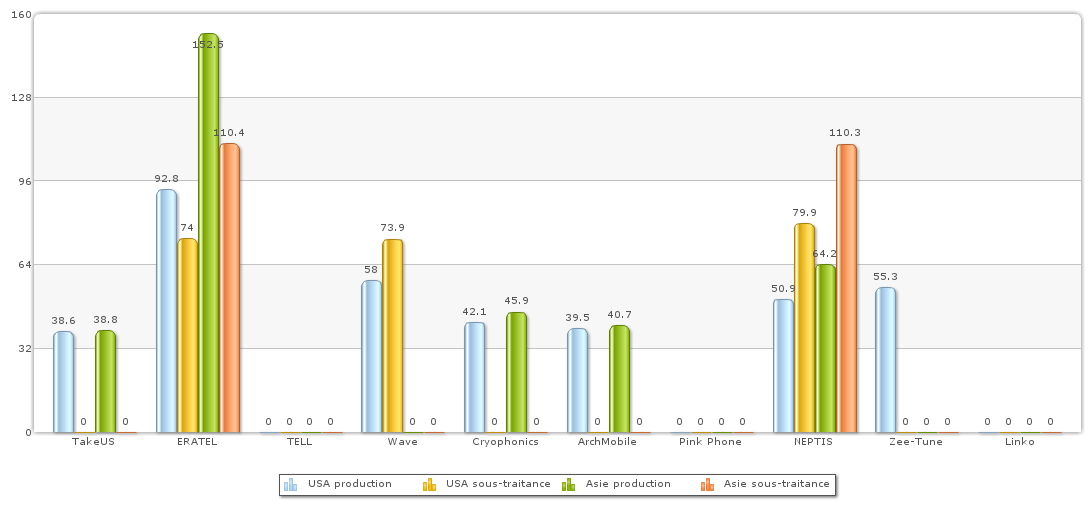
\includegraphics[width=\textwidth]{CoutTech3.png}
\end{figure}

\begin{figure}
  \caption{\label{coutTech4}Cout de production de la technologie 4}
  \centering
  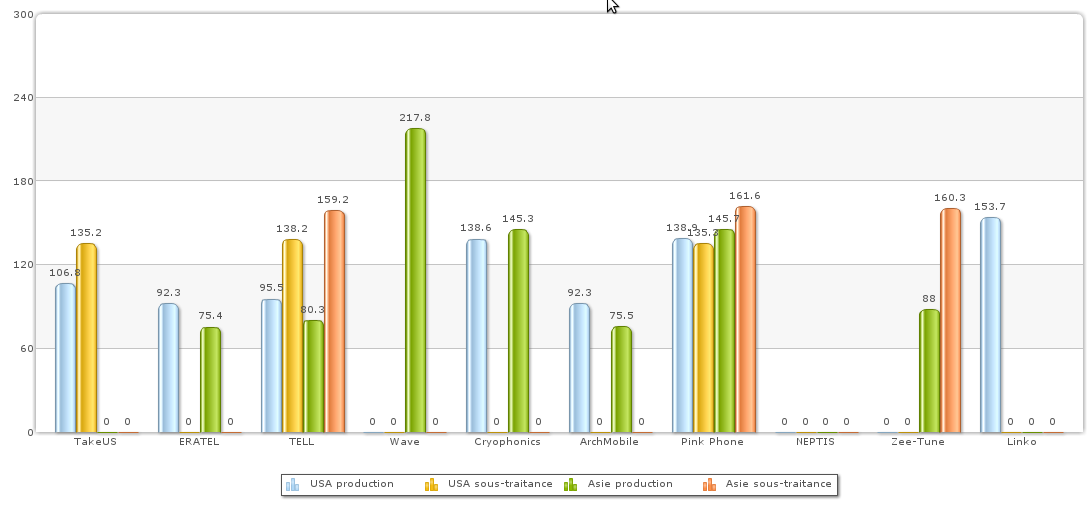
\includegraphics[width=\textwidth]{CoutTech4.png}
\end{figure}


\section{CONCLUSION : ANALYSE DE LA COMPÉTITION}
%%%%%%%%%%%%%%%% End main %%%%%%%%%%%%%%%%%
\end{document}
